% Feel free to contact me for any reason:
%% Email 1: zain.kamal@rutgers.edu
%% Email 2: z.kamal2021@gmail.com
%% Discord: alci#6038

%%%%%%%%%%%%%%%%%%%%%%%%%%%%%%%%%%%%%%%%%%%%%%%%%%%%%%%%%%%%%%%%%%%%%%%%%%%%%%%%%
\documentclass{article}
% Feel free to contact me for any reason:
%% Email 1: zain.kamal@rutgers.edu
%% Email 2: z.kamal2021@gmail.com
%% Discord: alci#6038

% Last updated 1/28/22

% Template based off of Justin Kim's (don't know where he got it from originally), but I've made a ton of edits. His soul lives on in random packages and commands I'm too lazy to comment out.


%%%%%%%%%%%%%%%%%%%%%%%%%%%%%%%%%%%%%%%%%%%%%%%%%%%%%%%%%%%%%%%%%%%%%%%%%%%%%%%%%%%%
%%% Default packages:

\usepackage[margin=1in]{geometry} 
\usepackage{amsmath,amsthm,amssymb,amsfonts, fancyhdr, color, comment, graphicx, environ}
\usepackage{xcolor}
\usepackage{mdframed}
\usepackage{bm}
\usepackage[shortlabels]{enumitem}
\usepackage{mathtools}
\usepackage{listings}
\usepackage{stmaryrd}
\usepackage{indentfirst}
\usepackage{hyperref}


%%%%%%%%%%%%%%%%%%%%%%%%%%%%%%%%%%%%%%%%%
%%% Pacakages I've added:

%% For Math 300 (Winter 2021):

\usepackage{mathdots} % for \iddots

\usepackage[ruled]{algorithm2e} % Algorithms
% NOTE: FIND A BETTER ALGORITHM PACKAGE, OR ATLEAST LEARN HOW TO USE THIS ONE BECAUSE DOUBLE INDENTING IS A FUCKING NIGHTMARE (or just import from mathcha?)
%% Example algorithm:
% \begin{center}
% 	\begin{minipage}{0.5\linewidth} % Adjust the minipage width to accomodate for the length of algorithm lines
% 		\begin{algorithm}[H]
% 			\KwIn{$(a, b)$, two floating-point numbers}  % Algorithm inputs
% 			\KwResult{$(c, d)$, such that $a+b = c + d$} % Algorithm outputs/results
% 			\medskip
% 			\If{$\vert b\vert > \vert a\vert$}{
% 				exchange $a$ and $b$ \;
% 			}
% 			$c \leftarrow a + b$ \;
% 			$z \leftarrow c - a$ \;
% 			$d \leftarrow b - z$ \;
% 			{\bf return} $(c,d)$ \;
% 			\caption{\texttt{FastTwoSum}} % Algorithm name
% 			\label{alg:fastTwoSum}   % optional label to refer to
% 		\end{algorithm}
% 	\end{minipage}
% \end{center}



%%%%%%%%%%%%%%%%%%%%%%%%%%%%%%%%%%%%%%%%%%%%%%%%%%%%%%%%%%%%%%%%%%%%%%%%%%%%%%%%%%%%
%%% Default commands:

\renewcommand{\vec}[1]{\mathbf{#1}}
	
\newcommand{\WidestEntry}{$lon_1$}%
\newcommand{\SetToWidest}[1]{\makebox[\widthof{\WidestEntry}]{#1}}%
\newcommand\tab[1][0.61cm]{\hspace*{#1}}
\newcommand{\nats}{\mathbb{N}}
\newcommand{\rats}{\mathbb{Q}}
\newcommand{\reals}{\mathbb{R}}
\newcommand{\Z}[1]{\mathbb{Z}_{#1}}
\newcommand{\BigO}[1]{\mathcal{O}(#1)}
\newcommand{\seq[1]}{(#1_n)}
\newcommand{\subseq[1]}{(#1_{n_k})}
\newcommand{\Lim}[2]{\lim \limits _{#1 \to #2}}
\newcommand{\Min}[2]{\min \{#1, #2\}}
\newcommand{\inv}{^{-1}}
\newcommand{\h}{^\text{th}}
\newcommand{\lrangle}[1]{\langle #1 \rangle}
\newcommand{\abs}[1]{\left\lvert #1 \right\rvert}

\DeclarePairedDelimiter{\ceil}{\lceil}{\rceil}
\DeclarePairedDelimiter{\floor}{\lfloor}{\rfloor}
\DeclareMathOperator{\supp}{supp}
\DeclareMathOperator{\rad}{rad}
\DeclareMathOperator*{\argmin}{arg\,min}
\DeclareMathOperator*{\argmax}{arg\,max}
\DeclareMathOperator*{\Var}{Var}
\DeclareMathOperator*{\Cov}{Cov}
\DeclareMathOperator*{\Corr}{Corr}
\DeclareMathOperator*{\Aut}{Aut}
\newcommand{\prob}[1]{\section*{Problem #1}}


%%%%%%%%%%%%%%%%%%%%%%%%%%%%%%%%%%%%%%%%%
%%% Commands I've added:

%% For Math 300 (Winter 2021):

\newcommand{\lrbrace}[1]{\{ #1 \}}
\newcommand{\powerset}{\mathcal{P}}
\newcommand{\ints}{\mathbb{Z}}

% Source/inspiration: https://tex.stackexchange.com/a/42728:
\newcommand{\numberthis}{\addtocounter{equation}{1}\tag{\theequation}\label{\theequation}}
    % Within an `align*` environment, put `\numberthis` after a line to number it. 
    % Access it with `\eqref{ [number of equation] }`
\newcommand{\numberthiswith}[1]{\addtocounter{equation}{1}\tag{\theequation}\label{#1}}
    % Within an `align*` environment, put `\numberthiswith{ [your_label] }` after a line to number it. 
    % Access it with `\eqref{ [your_label] }`



%%%%%%%%%%%%%%%%%%%%%%%%%%%%%%%%%%%%%%%%%%%%%%%%%%%%%%%%%%%%%%%%%%%%%%%%%%%%%%%%%%%%
%%% Default formatting:

\hypersetup{
    colorlinks=true,
    linkcolor=blue,
    filecolor=magenta,      
    urlcolor=blue,
}

\setlength{\parindent}{0cm}
\setlength{\parskip}{6pt}

\pagestyle{fancy}


%% Misc formatting additions

% make bullets with itemize much smaller
\newlength{\mylen}
\setbox1=\hbox{$\bullet$}\setbox2=\hbox{\tiny$\bullet$}
\setlength{\mylen}{\dimexpr0.5\ht1-0.5\ht2}
\renewcommand\labelitemi{\raisebox{\mylen}{\tiny$\bullet$}}


% Modified version of problem environment below
% \newenvironment{problem}[2][Problem]
%     { \begin{mdframed}[backgroundcolor=gray!5] \textbf{#1 #2} \\}
%     {  \end{mdframed}}
% \newenvironment{solution}{\textbf{Solution}\\}


%%%%%%%%%%%%%%%%%%%%%%%%%%%%%%%%%%%%%%%%%
%%% Formatting I've added:

%% Grey boxes for problem statements (note that I don't have a "solution" section):

% Problem environment, but shows "(a)" instead of "Problem a"
\newenvironment{problem}[2][]
    { \begin{mdframed}[backgroundcolor=gray!5] \textbf{#1 (#2)}}
    {  \end{mdframed}}
% Problem environment, but no "([input_char])" at all
\newenvironment{problem*}
    { \begin{mdframed}[backgroundcolor=gray!5] \\}
    {  \end{mdframed}}


% Example environment, currently identical to "problem" (Note: this is better written than the problem environment because I wrote it myself from scratch. Use this as an example for future new environments.)
\newcounter{example}[section]
\newenvironment{example}
    { 
        \refstepcounter{example}
        \begin{mdframed}[backgroundcolor=gray!5]
        \textbf{\\Example \thesection.\theexample:}
    }
    {\\ \end{mdframed}}


%%%%%%%%%%%%%%%%%%%%%%%%%%%%%%%%%%%%%%%%%%%%%%%%%%%%%%%%%%%%%%%%%%%%%%%%%%%%%%%%%%%%
% Misc things I've added




%%%%%%%%%%%%%%%%%%%%%%%%%%%%%%%%%%%%%%%%%%%%%
% Fill in the appropriate information below
\lhead{Zain Kamal}
% \rhead{Math 244 Spring 2022} % Moved to document
% \chead{\textbf{Homework 2}} % Moved to document
\begin{document}
\chead{\textbf{1. EM Waves}}
\rhead{Physics 228H}
%%%%%%%%%%%%%%%%%%%%%%%%%%%%%%%%%%%%%%%%%%%%%%%%%%%%%%%%%%%%%%%%%%%%%%%%%%%%%%%%%

\section{}

See dynalist notes, transfer eventually (just main results, derivations probably aren't necessary for anything ever at all)

\section{Energy of EM Waves: The Poynting Vector}

Recall that the ``energy density" of an electromagnetic field is the potential energy per volume:
\begin{equation}
u=\frac{U}{V} =\tfrac{1}{2} \epsilon _{0} E^{2} +\tfrac{1}{2\mu _{0}} B^{2} ,
\end{equation}
which when combined with $E=cB$ from the previous lecture, yields:
\begin{align*}
u & =\tfrac{1}{2} \epsilon _{0} E^{2} +\tfrac{1}{2\mu _{0}}\tfrac{E^{2}}{c^{2}} ,\\
 & \left[ use\ c=\tfrac{1}{\sqrt{\epsilon _{0} \mu _{0}}}\right]\\
 & =\tfrac{1}{2} \epsilon _{0} E^{2} +\tfrac{1}{2\mu _{0}} \epsilon _{0} \mu _{0} E^{2}\\
 & =\epsilon _{0} E^{2} .
\end{align*}
So $E$ and $B$ have the same energy density at any given moment in time ($u_{E} =u_{B}$). Neat!

\

Recall that for the plane wave, $\vec{E} \times \vec{B} =\vec{v}$. So we consider an EM plane wave that travels some distnace:

\begin{figure}[htp]
    \centering
    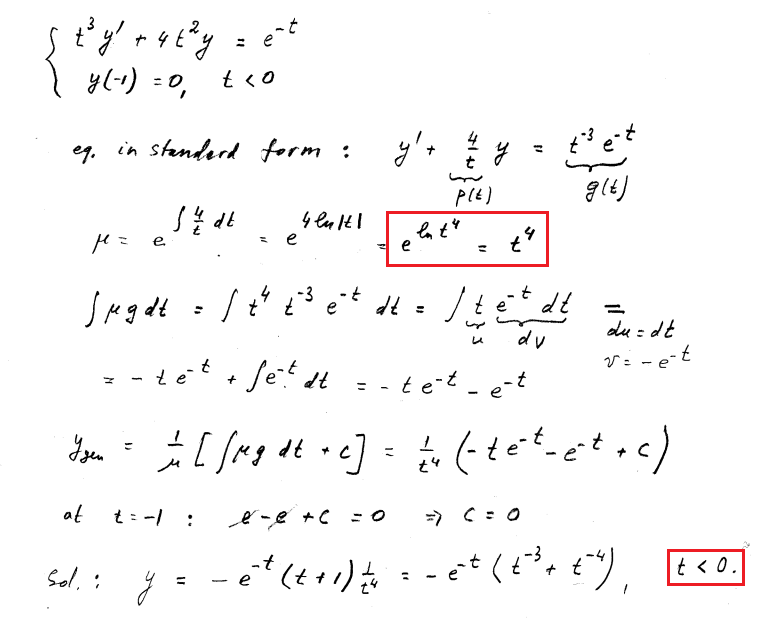
\includegraphics[width=6cm]{images/3.1.png}
\end{figure}

By taking the derivative of equation (1), we find:
\begin{align*}
dU & =u\cdot dV\\
 & =\left( \epsilon _{0} E^{2}\right)( A\cdot c\ dt)\\
\Rightarrow \frac{1}{A} \cdot \frac{dU}{dt} & =\epsilon _{0} cE^{2}\\
 & [ use\ E=cB]\\
 & =\epsilon _{0} cE( cB)\\
 & =\epsilon _{0} c^{2} EB\\
 & \left[ use\ c=\tfrac{1}{\sqrt{\epsilon _{0} \mu _{0}}}\right]\\
 & =\tfrac{1}{\mu _{0}} EB.
\end{align*}
If we define $S:=\frac{1}{A} \cdot \frac{dU}{dt}$, we can promote $S$ to a vector:
\begin{equation}
\boxed{\vec{S} =\tfrac{1}{\mu _{0}} \ \vec{E} \times \vec{B} ,}
\end{equation}
which we call the \underline{Poynting Vector}, representing the energy flowing through EM waves.



\textit{Remark:} This better describes how energy in an AC circuit flows in one direction, in spite of the electron flow / E-field constantly reversing directions. This \href{https://www.veritasium.com/videos/2021/11/19/the-big-misconception-about-electricity}{Veritasium video} gives a great visualization of how the it's the fields transfer energy, not the electrons. 

\

\


Now consider some EM plane wave moving in the $\hat{x}$\textit{ direction}, given by $\begin{cases}
\vec{E} =E_{0}\cos( kx-\omega t)\hat{y}\\
\vec{B} =B_{0}\cos( kx-\omega t)\hat{z}
\end{cases}$.

We ``reverse" the wave to move in $-\hat{x}$\textit{ direction} by flipping $\vec{B}$ and changing the phase such that as $t$ increases, the $\cos$ wave shifts to the left ($-x$ direction): $\begin{cases}
\vec{E} =E_{0}\cos( kx+\omega t)\hat{y}\\
\vec{B} =B_{0}\cos( kx+\omega t)( -\hat{z})
\end{cases}$.

We plug these $\vec{E}$ and $\vec{B}$ into the Poynting Vector from (2) to get
\begin{align*}
\vec{S} & =\tfrac{1}{\mu _{0}} E_{0} B_{0}\cos^{2}( kx-\omega t)\hat{x} .
\end{align*}
Note that this is positive for all $t$, which solidifies the notion of energy transfer (if it were oscillating back and forth, it would cancel out). 



The average of $\cos^{2}$ is a half, so the average of the Poynting vector becomes:
\begin{equation*}
\boxed{\langle S\rangle =\tfrac{1}{2\mu _{0}} E_{0} B_{0} .}
\end{equation*}

\

\hline

%%%%%%%%%%%%%%%%%%%%%%%%%%%%%%%%%%%%%%%%%%%%%%%%%%%%%%%%%%%%%%%%%%%%%%%%%%%%%%%%%
\end{document}